Although the primary goal of our paper is to \textit{understand} what drives memorability of objects in a scene, the current work also makes available the very first dataset containing the ground truth memorability of constituent objects from a highly diverse image set. In this section, we show that our dataset can serve as a  benchmark for the purpose of object memorability prediction by making use of the ground truth memorability maps constructed from experimental data.

\textbf{Baseline models:} As a first step, we propose a simple baseline model that utilizes a conv-net \cite{krizhevsky12}, \cite{jia14} trained on the ImageNet database \cite{deng09}. Since object categories play an important role in determining object memorability (\ref{sec:obLabel}), and deep learning models have recently been shown to achieve state-of-the-art results in various other recognition tasks, including object recognition and object categorization (cite papers here), we believe that this simple model can serve as a good initial baseline for object memorability prediction. We first generated object segments by using MCG, a generic object proposal method proposed in \cite{arbelaez14}. Next, we trained an SVR using $6$-fold cross-validation on the original segments to map deep features to memorability scores. We then used this model to predict the memorability scores for the top K ($K=20$) segments (obtained via the ranking scores provided by the MCG algorithm) for each image. After obtaining the predicted memorability scores, the memorability maps were generated by averaging the top $K$ segments at the pixel level. Since image features like SIFT \cite{lowe04} and HOG \cite{dalal05} have previously been shown to achieve good performance in predicting image memorability, we built a second baseline model using these features for comparison. Training and testing of this model was performed similar to the deep-net baseline model.

\textbf{Evaluation: } To evaluate the accuracy of the predicted memorability maps, we computed the rank correlation between the mean predicted memorability score inside each of the original object segments and their ground truth memorability scores. From figure \ref{fig:benchmark}, we first note that our deep-net baseline model performs considerably well ($\rho = 0.39$), reaching a level of performance that approaches  that of human consistency. In contrast, the baseline model trained using HOG and SIFT features exhibits much lower overall performance ($\rho = 0.27$). We also included $8$ state-of-the-art-saliency methods \textbf{gb} \cite{gb}, \textbf{aim} \cite{aim}, \textbf{dv} \cite{dv}, \textbf{it} \cite{it}, \textbf{gc} \cite{gc}, \textbf{pc} \cite{pc}, \textbf{sf} \cite{sf}, and \textbf{ft} \cite{ft} to our comparison (some of these are the top performing methods according to benchmarks in \cite{borji13}, \cite{borji12}). Saliency maps generated from these methods are likely to have some degree of overlap with memorability and are therefore worth comparing to our baseline, especially given the absence of alternative memorability prediction methods. Results from figure \ref{fig:benchmark}) show that the HOG+SIFT baseline is outperformed by most saliency methods. Thus, even though models using these features have previously demonstrated high predictive power in predicting image memorability, they may not be as well  suited for the task of predicting object memorability. The deep-net baseline model performs better than all other saliency methods and only \textbf{pc} ($\rho=0.38$), \textbf{sf} ($rho=0.37$), and \textbf{gb} ($rho=0.36$) show performance comparable to the model. A common factor between these saliency methods is that they explicitly add center bias to their implementation, which could be a  part of the reason for their favorable performance. Despite this, the deep-net model performs comparably against them and is potentially much better suited for memorability prediction. Thus, we recommend in the future, memorability algorithms compare their methods against our deep-net baseline. While the deep-net model performed fairly well, part of the performance of such a model is dependent on the quality of the segmentations used. For this reason, we also consider the upper bound of our current predictive power by showing the results for our model containing predictions on the original segments (Figure \ref{fig:benchmark}). Interestingly, the accuracy of this model is very high and close to human performance ($\rho = 0.7$). This demonstrates that the deep-net model has high predictive ability that is suppressed most heavily by constraints of the segmentation task. As the main insight of our evaluation, we have have demonstrated that deep features serve as strong predictors of memorability and selection of higher quality segments can potentially lead to improved memorability prediction algorithms.

\begin{figure}[t]
\centering
\subfigure{\centering 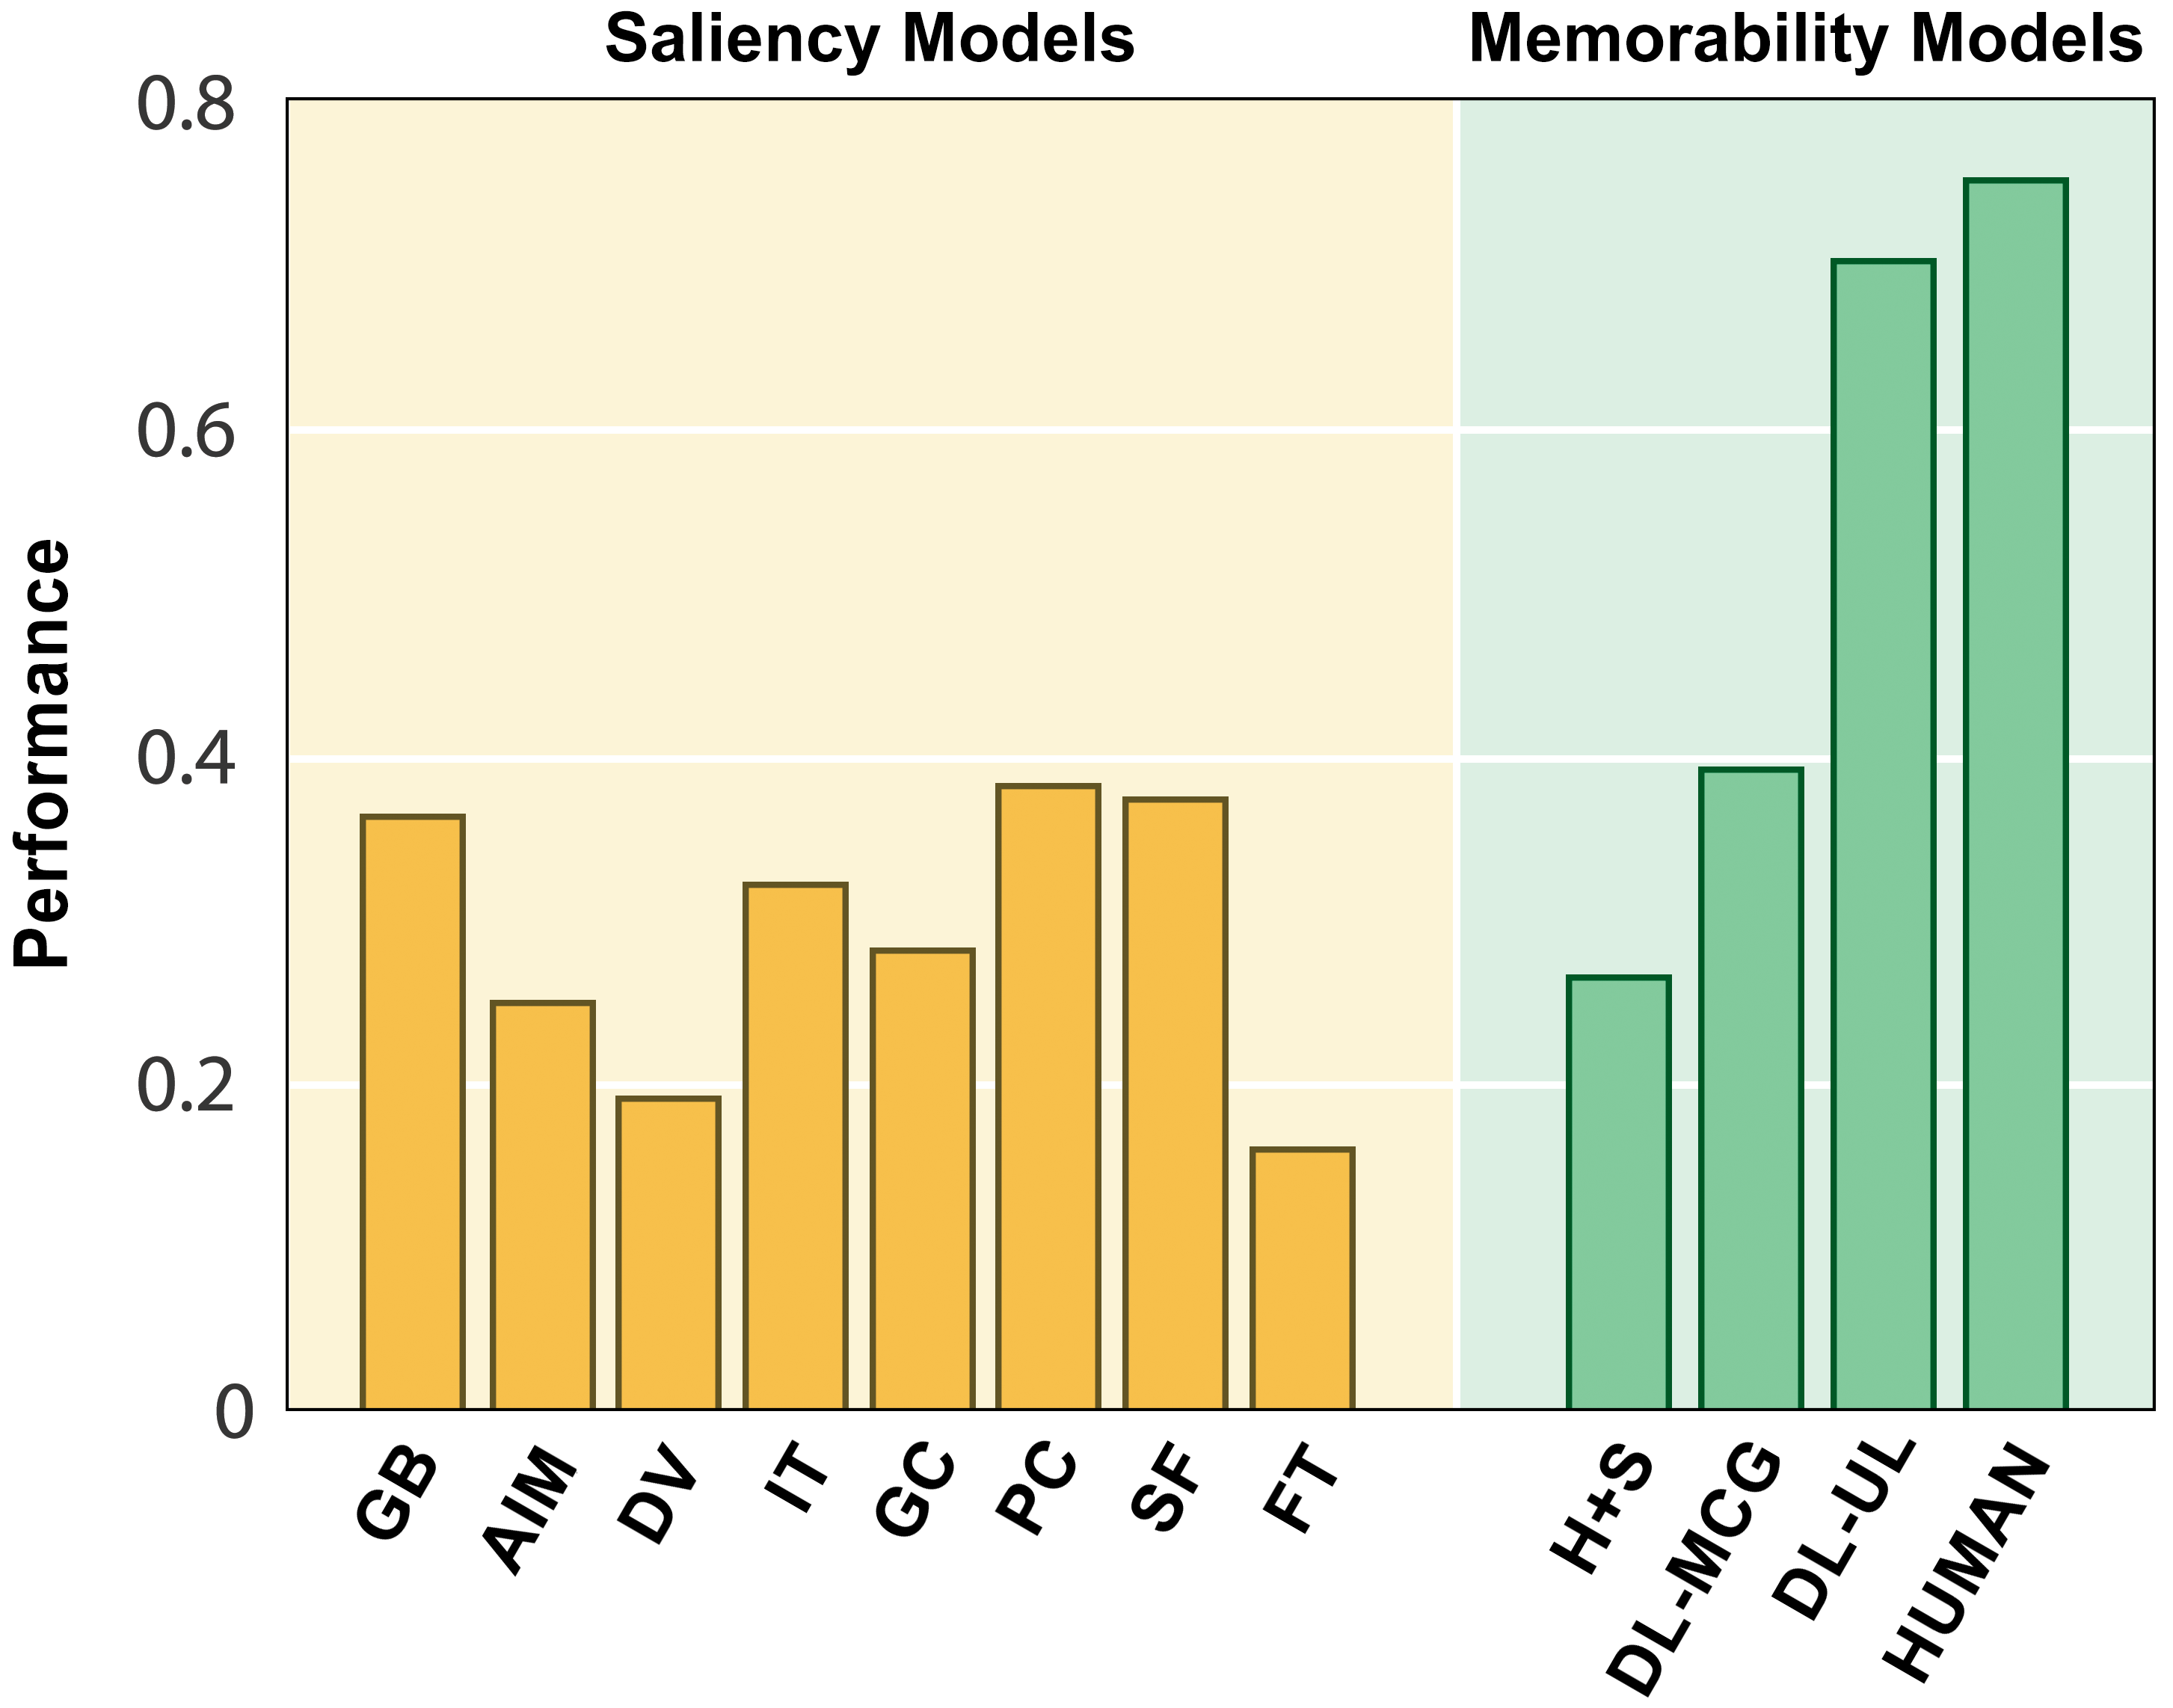
\includegraphics[width=0.4\textwidth]{figures/results/benchmark/comparison.png}}
\vspace{-5mm}\caption{\footnotesize\textbf{Main task.} add-in later. }\label{fig:benchmark}
\end{figure} 